%  LaTeX support: latex@mdpi.com 
%  For support, please attach all files needed for compiling as well as the log file, and specify your operating system, LaTeX version, and LaTeX editor.

%=================================================================
\documentclass[mathematics,article,submit,moreauthors]{Definitions/mdpi} 

%=================================================================
% MDPI internal commands - do not modify
\firstpage{1} 
\makeatletter 
\setcounter{page}{\@firstpage} 
\makeatother
\pubvolume{1}
\issuenum{1}
\articlenumber{0}
\pubyear{2026}
\copyrightyear{2026} 
%\externaleditor{Firstname Lastname} % More than 1 editor, please add `` and '' before the last editor name
\datereceived{ } 
\daterevised{ } % Comment out if no revised date
\dateaccepted{ } 
\datepublished{ } 
%\datecorrected{} % For corrected papers: "Corrected: XXX" date in the original paper.
%\dateretracted{} % For retracted papers: "Retracted: XXX" date in the original paper.
%\doinum{} % Used for some special journals, like molbank
%\pdfoutput=1 % Uncommented for upload to arXiv.org
%\CorrStatement{yes}  % For updates
%\longauthorlist{yes} % For many authors that exceed the left citation part
%\IsAssociation{yes} % For association journals

%=================================================================
% Add packages and commands here. The following packages are loaded in our class file: fontenc, inputenc, calc, indentfirst, fancyhdr, graphicx, epstopdf, lastpage, ifthen, float, amsmath, amssymb, lineno, setspace, enumitem, mathpazo, booktabs, titlesec, etoolbox, tabto, xcolor, colortbl, soul, multirow, microtype, tikz, totcount, changepage, attrib, upgreek, array, tabularx, pbox, ragged2e, tocloft, marginnote, marginfix, enotez, amsthm, natbib, hyperref, cleveref, scrextend, url, geometry, newfloat, caption, draftwatermark, seqsplit
% cleveref: load \crefname definitions after \begin{document}

%=================================================================
% Please use the following mathematics environments: Theorem, Lemma, Corollary, Proposition, Characterization, Property, Problem, Example, ExamplesandDefinitions, Hypothesis, Remark, Definition, Notation, Assumption
%% For proofs, please use the proof environment (the amsthm package is loaded by the MDPI class).

%=================================================================
% Full title of the paper (Capitalized)
\Title{Beyond Linear Trade-offs in Context-Aware Decision Support: Non-Linear Aggregation and Rank Stability Analysis}

% Author Orchid ID: enter ID or remove command 
\newcommand{\orcidauthorA}{0000-0003-3267-6753} % Add \orcidA{} behind the author's name
\newcommand{\orcidauthorB}{0009-0002-0183-7905} % Add \orcidB{} behind the author's name
\newcommand{\orcidauthorC}{0000-0002-7653-1452} % Add \orcidB{} behind the author's name

% Authors, for the paper (add full first names)
\Author{Pavel Novoa-Hern\'andez$^{1,*}$\orcidA{}, Mariia Godz$^{2}$\orcidA{} and David A. Pelta$^{2}$\orcidC{}}

%\longauthorlist{yes}

% MDPI internal command: Authors, for metadata in PDF
\AuthorNames{Pavel Novoa-Hern\'andez, Mariia Godz and David A. Pelta}

%\longauthorlist{yes}

% Affiliations / Addresses (Add [1] after \address if there is only one affiliation.)
\address{%
$^{1}$ \quad Dept. Computer Engineering and Systems, Universidad de La Laguna; pnovoahe@ull.edu.es\\
$^{2}$ \quad Dept. Computer Science and Artificial Intelligence, Universidad de Granada; \{mariiagodz,dpelta\}@ugr.es}

% Contact information of the corresponding author
\corres{Correspondence:pnovoahe@ull.edu.es}

% Current address and/or shared authorship
%\firstnote{Current address: Affiliation.}  
% Current address should not be the same as any items in the Affiliation section.

%\secondnote{These authors contributed equally to this work.}
% The commands \thirdnote{} till \eighthnote{} are available for further notes.

%\simplesumm{} % Simple summary

%\conference{} % An extended version of a conference paper

% Abstract (Do not insert blank lines, i.e. \\) 
\abstract{Hybrid automated decision-making systems increasingly combine machine-learning probability or confidence scores with contextual rules, expert knowledge, or organizational constraints. In such settings, the aggregation operator is not a technical detail: it determines whether predictive evidence may compensate for contextual non-compliance, or whether contextual requirements act as binding limits. Recent fuzzy multi-criteria decision-making research has produced many non-linear aggregation operators, but the literature provides little empirical evidence on their systemic effects, including policy violations, rank reversals, and the propagation of contextual noise. This paper studies these effects within the CADEMAS framework by comparing linear aggregation, the conjunctive minimum, and a weighted geometric operator. We first establish formal conditions under which aggregation semantics induce rank reversals or preserve predictive order under contextual homogeneity. We then run Monte Carlo simulations that stress-test resource allocation, targeted predictive overconfidence, and noisy contextual assessments. The results show that linear aggregation is efficient within a limited compliance region but can admit vetoed cases under high predictive weight, whereas the non-linear operators provide a structural firewall against zero-context alternatives. Under contextual noise, the minimum operator shows higher rank stability than the linear rule. Finally, a 100-employee machine-learning-based CADEMAS attrition cohort with Top-$K$ prioritization ($K = 10$) illustrates how $A_L$ at low, balanced, and high $\lambda$ reorders cases when cooperative risk and context score are heterogeneous, including outsiders who enter the intervention tier under non-baseline settings and a policy violation under risk-dominated linear integration. The study supports operator selection as a governance decision rather than a purely mathematical modeling choice.}

% Keywords
\keyword{automated decision-making; CADEMAS; fuzzy aggregation operators; multi-criteria decision making; rank stability; contextual governance; employee attrition} 

%%%%%%%%%%%%%%%%%%%%%%%%%%%%%%%%%%%%%%%%%%
\begin{document}


\section{Introduction}

Automated Decision-Making (ADM) systems are now used in settings where recommendations have economic, organizational, and ethical consequences. Machine learning has improved the ability to estimate risks and anticipate events, but a good prediction is not always an actionable decision. A hospital, a company, or a public agency may need to respect resource limits, institutional policies, safety constraints, or expert-defined priorities before acting on a model output. This is why many decision-support systems are moving from purely predictive pipelines toward hybrid architectures that combine data-driven evidence with rules, contextual information, and domain knowledge \citep{Kierner2023,Rahman2025,PerezDominguez2024}.

This shift creates a methodological problem that is easy to overlook. Once predictive evidence and contextual knowledge coexist, the final recommendation depends on how both signals are integrated. The aggregation rule therefore becomes part of the policy. It decides whether a high predicted risk can compensate for weak contextual support, whether a contextual veto must dominate the model, or whether the system should operate somewhere between those two extremes.

\citet{NovoaHernandez2026} proposed the Cooperative Automated Decision-Making System (CADEMAS) framework to make this separation explicit. CADEMAS organizes heterogeneous ADM units within a layered architecture: predictive or automated components produce partial evidence, an integration layer combines their outputs, and a contextual modulator evaluates the result under organizational or institutional criteria. In the machine-learning-based CADEMAS (CADEMAS-ML) employee-attrition instantiation of \citet{Godz2026}, for example, machine-learning models estimate the probability that an employee will leave, while fuzzy contextual rules encode retention priorities such as strategic fit, development potential, or organizational vulnerability.

Existing CADEMAS instantiations \citep{NovoaHernandez2026, Godz2026}, however, usually combine predictive risk and context through a linear convex rule. The appeal is clear: the parameter is interpretable, and the resulting score is easy to explain. Yet linearity also imposes a strong assumption. It treats prediction and context as fully compensatory dimensions. A sufficiently high risk score may offset poor contextual compatibility, and strong contextual support may offset weak predictive evidence. This is not necessarily wrong, but it is not neutral. In domains where contextual information represents a regulation, a safety requirement, or a fairness constraint, unrestricted compensation may lead to recommendations that are numerically plausible but institutionally unacceptable.

The fuzzy Multi-Criteria Decision-Making (MCDM) literature offers many alternatives to linear averaging. Ordered weighted, geometric, t-norm-based, Frank, Einstein, Aczel--Alsina, Dombi, and Diophantine fuzzy operators have been developed to represent different forms of interaction among criteria \citep{Yager1988,Grabisch1996,Tan2009,Mahmood2022,Iampan2021,Riaz2021,Riaz2022,Riaz2021a,Jeevitha2023}. This literature is mathematically rich. It establishes properties such as boundedness, monotonicity, idempotency, and sensitivity to operator parameters. It also shows that aggregation choices can affect rankings in concrete decision problems.

What remains less developed is the systemic evaluation of these operators. \citet{Aires2018} show that rank reversal is a long-standing reliability problem in MCDM, and recent comparisons suggest that ranking stability can vary substantially across method architectures \citep{Amman2025,Kizielewicz2025}. Still, the available evidence says little about the questions that matter for hybrid ADM systems: how often does an operator allow policy-violating cases into a resource-constrained top tier? Can a non-linear operator insulate a decision process from localized predictive overconfidence? How does fuzzy contextual noise propagate into final rankings? The literature has largely prioritized the construction of new operators and application examples over controlled benchmarking of such effects.

This paper addresses that gap for the CADEMAS setting. We do not propose another aggregation operator. Instead, we treat the aggregation stage as the mathematical place where governance semantics are encoded. A linear rule represents a fully compensatory policy; a conjunctive minimum represents a strict non-compensatory policy; a weighted geometric mean offers a non-linear intermediate regime with a hard zero boundary. We analyze how these regimes reshape the decision space, modify rankings, and respond to contextual uncertainty.

The empirical part of the paper has two layers. First, we run controlled Monte Carlo simulations to examine three aspects of operator behavior: policy compliance under increasing predictive weight, resilience to localized model overconfidence, and rank stability under noisy fuzzy context. Second, we apply the same operators to the full 100-case CADEMAS-ML employee-attrition cohort and select a Top-$K$ tier with $K = 10$ (10\% of the population). The case study does not replace the simulations; it shows how the same semantics appear in a concrete prioritization task when $\lambda$ shifts toward context or cooperative risk, when outsiders enter the intervention tier under non-baseline integration settings, and when a context-vetoed employee can enter the Top-$K$ tier under risk-dominated linear integration.

The main contributions of this work are fivefold:

\begin{itemize}
\item We formulate the integration of predictive risk and fuzzy contextual knowledge within CADEMAS as a generalized aggregation problem.

\item We study representative aggregation regimes with distinct compensation semantics: linear, conjunctive minimum, and weighted geometric integration.

\item We characterize how aggregation semantics induce rank reversals or preserve predictive ordering under contextual homogeneity.

\item We evaluate systemic effects that are underreported in the fuzzy MCDM literature: policy violations, targeted overconfidence, and noise propagation in prioritization rankings.

\item We validate the interpretation on the 100-case CADEMAS-ML employee-attrition cohort, comparing $A_L$ at $\lambda \in \{0.1, 0.5, 0.9\}$ with $A_T^{\min}$ and $A_G$, and showing how operator choice and $\lambda$ jointly reshape the Top-$K$ tier, including ghost entrants outside the baseline list.
\end{itemize}

The remainder of the paper is organized as follows. Section~\ref{sect:cademas} introduces the CADEMAS framework and its instantiations. Section~\ref{sect:nonlinear_integration} formalizes the aggregation models and their structural properties. Section~\ref{sect:simulation} presents the simulation study and its findings. Section~\ref{sect:real_example} applies the operators to a published employee-attrition instantiation. Section~\ref{sect:conclusions} summarizes the main conclusions, limitations, and directions for future work.



\section{The CADEMAS Framework and Its Instantiations}\label{sect:cademas}

\citet{NovoaHernandez2026} define CADEMAS (Cooperative Automated Decision-Making Systems) as a general framework for designing context-aware decision support systems in which heterogeneous Automated Decision-Making (ADM) components cooperate to produce a unified decision outcome. Unlike conventional ensemble methods, where multiple predictive models are combined solely to improve predictive performance, CADEMAS explicitly separates predictive inference from contextual governance. Predictive evidence and institutional knowledge are therefore treated as complementary sources of information that jointly determine the final recommendation.

Formally, a CADEMAS instance is represented by the tuple
\begin{equation}
\mathcal{S}=
\langle I, U, O, K, T \rangle,
\end{equation}
where $I$ denotes the Input Manager, $U$ the set of Automated Decision-Making units, $O$ the Decision Integration Layer, $K$ the Contextual Modulator, and $T$ the universe of admissible data representations. In practical terms, $U$ is where machine-learning or rule-based models produce partial scores, $O$ is where those scores are combined, and $K$ is where organizational policy, expert knowledge, or fuzzy contextual rules enter the workflow. The architecture is intentionally generic and independent of any particular predictive model or contextual representation.

The ADM units generate partial decision signals from the available information, while the Decision Integration Layer harmonizes these heterogeneous outputs into a unified decision object. The Contextual Modulator then adjusts this preliminary outcome according to organizational policies, regulatory requirements, expert knowledge, or other contextual factors. This layered organization preserves a clear separation between what the data suggest and what the institution is willing to prioritize.

Recent applications have instantiated this architecture in domains where machine learning predictions must be reconciled with institutional decision policies. The employee attrition scenario presented by \citet{Godz2026} is a representative CADEMAS-ML application: predictive models estimate the probability that an employee voluntarily leaves the organization, whereas fuzzy contextual rules encode organizational priorities regarding employee retention. Similarly, in the SME insolvency risk application, predictive models estimate financial distress while contextual rules incorporate business and organizational considerations into the prioritization process.

Although these applications differ in domain and predictive models, they share a common decision structure. For each decision case $i$, the predictive subsystem produces a normalized cooperative risk score
\begin{equation}
R_i \in [0,1],
\end{equation}
which aggregates the outputs of one or more ADM units. In CADEMAS-ML, each unit contributes the predicted probability or confidence assigned to the positive class of interest (e.g., voluntary attrition), and $R_i$ denotes their cooperative combination. The contextual modulator computes a normalized contextual satisfaction degree
\begin{equation}
Q_i \in [0,1],
\end{equation}
also referred to as the \emph{context score}, which measures how strongly the active contextual scenario supports prioritizing case $i$ (e.g., strategic retention fit under a digital-transformation scenario encoded by fuzzy rules). Independently of the application domain, the integration layer must therefore construct a prioritization function
\begin{equation}
P_i = A(R_i,Q_i),
\end{equation}
where $A$ denotes an aggregation operator combining predictive evidence and contextual information. The final ranking over cases, and hence the Top-$K$ intervention list, follows directly from these scores.

Existing CADEMAS instantiations have adopted linear convex aggregation for $A$. In this work, we abstract the integration stage from any specific mechanism and study how different aggregation semantics reshape prioritization. The operator $A$ becomes the central design choice through which CADEMAS encodes compensatory, veto-based, or intermediate governance policies.


\section{Non-Linear Integration of Predictive Risk and Fuzzy Context}
\label{sect:nonlinear_integration}

We now formalize how predictive risk and fuzzy contextual knowledge are combined within CADEMAS. We first examine the standard linear integration scheme, introduce representative non-linear alternatives, and characterize the ranking structure that determines which cases enter the prioritized tier.

\subsection{The Limits of Linear Convex Combination}
\label{subsect:linear_limits}

Existing CADEMAS instantiations, including applications in employee attrition and SME insolvency risk assessment, typically integrate predictive and contextual information through a linear convex combination:
\begin{equation}
P_i = \lambda R_i + (1 - \lambda) Q_i, \quad \lambda \in [0,1],
\end{equation}
where $\lambda$ controls the relative weight of the predictive layer in the final score. In CADEMAS-ML, this parameter is exposed to domain experts as a trade-off slider between cooperative risk ($R_i$) and context score ($Q_i$).

This formulation is fully compensatory. Consider two alternatives $i$ and $j$ such that $R_i > R_j$ and $Q_i < Q_j$. Under linear aggregation, the ordering between $i$ and $j$ depends solely on $\lambda$. A deterioration in contextual compatibility can always be offset by an increase in predictive risk, and vice versa. For CADEMAS, this means that a case with weak contextual support may still rank above a better-aligned peer if its predicted risk is sufficiently high.

The compensatory structure follows from constant partial derivatives:
\[
\frac{\partial P_i}{\partial R_i} = \lambda, \quad \frac{\partial P_i}{\partial Q_i} = 1 - \lambda,
\]
so the marginal rate of substitution between prediction and context does not change with the scores themselves. Iso-priority contours in the $(R_i, Q_i)$ plane are therefore straight lines. In settings where contextual information represents a safety requirement, a fairness constraint, or a hard organizational veto, unrestricted compensation may produce recommendations that are numerically high but institutionally unacceptable.

\subsection{Non-Linear Aggregation in CADEMAS}
\label{subsect:nonlinear_aggregators}

We do not propose new aggregation operators. We adopt well-established families from fuzzy connectives and MCDM that encode distinct compensation semantics \citep{Zimmermann1980,Klement1996}. Each choice of $A$ defines a different policy reading for the CADEMAS integration layer:
\begin{equation}
A: [0,1]^2 \rightarrow [0,1],
\end{equation}
with monotonicity and boundary conditions $A(0,0)=0$ and $A(1,1)=1$.

\begin{enumerate}
\item \emph{Conjunctive (non-compensatory) regime.} Classical fuzzy set intersection is modeled by operators such as the minimum and the algebraic product. In both cases, a low score on one dimension cannot be offset by a high score on the other \citep{Zimmermann1980,Klement1996}:
\begin{equation}
A_T^{\min}(R_i, Q_i) = \min(R_i, Q_i),
\end{equation}
\begin{equation}
A_T^{\prod}(R_i, Q_i) = R_i \cdot Q_i.
\end{equation}
In CADEMAS, the minimum acts as a contextual gate: the final priority cannot exceed the weaker signal. If $Q_i = 0$, then $P_i = 0$ regardless of $R_i$, which formalizes an institutional veto at the integration layer. This reading is consistent with non-compensatory aggregation in composite indicators and policy scoring \citep{Natoli2024,Blancas2024}. The algebraic product shares the same zero-absorption property but is less severe than the minimum for intermediate values.

For completeness, we note that the disjunctive (permissive) regime, represented by the maximum, would allow either dimension to dominate the aggregated score \citep{Zimmermann1980,Klement1996}:
\begin{equation}
A_S(R_i, Q_i) = \max(R_i, Q_i).
\end{equation}
This regime emphasizes the most favorable signal and suits exploratory settings. However, in the CADEMAS governance context, where contextual non-compliance should limit prioritization, the maximum is not appropriate because a vetoed case with $Q_i = 0$ would still receive $P_i = R_i$, allowing predictive risk alone to place institutionally excluded alternatives in the top tier. Therefore, we do not consider the maximum in the remainder of this work.

\item \emph{Non-linear compensatory regime.} Intermediate behavior between full compensation and strict non-compensation is often modeled by the weighted geometric mean \citep{Zimmermann1980,Turksen1992,Krejci2018,Mohammadi2023,Natoli2024}:
\begin{equation}
A_G(R_i, Q_i) = R_i^{\lambda} Q_i^{1-\lambda}, \quad \lambda \in [0,1].
\end{equation}
Unlike linear aggregation, this operator penalizes imbalance between $R_i$ and $Q_i$ while still allowing partial compensation. Recent composite-indicator work describes the geometric mean as occupying exactly this middle ground: less substitutable than the arithmetic mean, but not as rigid as a minimum operator \citep{Blancas2024,Natoli2024}. For CADEMAS, it offers a softer alternative to the minimum: contextual non-compliance reduces priority sharply but does not necessarily zero it unless $Q_i = 0$.

\end{enumerate}

\subsection{Rank Formulation and Structural Properties}
\label{subsect:rank_properties}

Given a set of decision alternatives $X = \{1,\dots,n\}$, each alternative $i \in X$ is assigned a score $P_i = A(R_i, Q_i)$, where $R_i \in [0,1]$ is the cooperative risk score and $Q_i \in [0,1]$ is the context score (contextual satisfaction degree). We define the aggregated score vector $\mathbf{P}(A) = (P_1, \dots, P_n)$ and the ranking function
\begin{equation}
\pi_A = \operatorname{argsort}_{i \in X} \, P_i,
\end{equation}
such that $P_{\pi_A(1)} \geq P_{\pi_A(2)} \geq \cdots \geq P_{\pi_A(n)}$. The mapping $A \rightarrow \mathbf{P}(A) \rightarrow \pi_A$ is the operational output of the CADEMAS integration layer: it determines which cases appear in the Top-$K$ intervention tier and in what order.

This ranking $\pi_A$ is the primary object of analysis in the subsequent sections. To interpret the empirical results, we establish two structural properties that govern how the choice of $A$ affects the stability of $\pi_A$ relative to the initial predictive ordering. We focus on \emph{rank reversal}, the situation where the final ranking inverts the order suggested solely by cooperative risk $R$.

Let $i, j \in X$ be two alternatives such that the predictive layer identifies $i$ as strictly riskier than $j$ ($R_i > R_j$). In a purely data-driven CADEMAS configuration, $i$ would always rank above $j$. The following propositions characterize when contextual evaluation $Q$ can reverse that order, depending on the semantic regime of $A$.

\begin{Proposition}[Policy-Driven Veto and Forced Rank Reversal]
\label{prop:rank_reversal}
The following results characterize the conditions under which the aggregation mechanism induces rank reversals under linear and non-linear regimes:

\begin{enumerate}
\item Under linear convex aggregation $A_L$ with trade-off parameter $\lambda \in (0,1)$, a rank reversal occurs ($P_j > P_i$) if and only if the contextual advantage of alternative $j$, defined as $\Delta Q = Q_j - Q_i$, satisfies:
\begin{equation}
\Delta Q > \frac{\lambda}{1-\lambda}(R_i - R_j).
\end{equation}

\item Under a strict conjunctive aggregator $A_T$ (which includes both the minimum $A_T^{\min}$ and the algebraic product $A_T^{\prod}$), if the contextual score of the disadvantaged alternative is zero ($Q_i = 0$) and the other alternative has strictly positive risk and context ($R_j > 0, Q_j > 0$), then a rank reversal is guaranteed: $P_j > P_i$, independently of the magnitude of $R_i$. This holds because $A_T(R_i, 0) = 0$ and $A_T(R_j, Q_j) > 0$.

\item Under the non-linear compensatory regime modeled by the weighted geometric mean $A_G$, assuming strictly positive inputs, a rank reversal occurs ($P_j > P_i$) if and only if the logarithmic ratio of contextual advantage satisfies:
\begin{equation}
\ln\left(\frac{Q_j}{Q_i}\right) > \frac{\lambda}{1-\lambda} \ln\left(\frac{R_i}{R_j}\right).
\end{equation}
\end{enumerate}
\end{Proposition}

\begin{proof}
For part (1), we establish the equivalence by starting from the rank reversal condition:
$$P_j > P_i \iff \lambda R_j + (1-\lambda) Q_j > \lambda R_i + (1-\lambda) Q_i.$$
Rearranging the terms (a strictly reversible algebraic operation) yields:
$$\iff (1-\lambda)(Q_j - Q_i) > \lambda (R_i - R_j).$$
Given $\Delta Q = Q_j - Q_i$, and since $\lambda \in (0,1)$ ensures $(1-\lambda) > 0$, we can divide both sides by $(1-\lambda)$ without altering the inequality's direction or the logical equivalence:
$$\iff \Delta Q > \frac{\lambda}{1-\lambda}(R_i - R_j).$$
This establishes both the necessary and sufficient conditions for the rank reversal under linear aggregation.

For part (2), we note that any strict conjunctive operator $A_T$ satisfies $A_T(x,0)=0$ and $A_T(x,y)>0$ whenever $x>0$ and $y>0$. Since $Q_i=0$, we have $P_i = A_T(R_i,0)=0$. Given $R_j>0$ and $Q_j>0$, it follows that $P_j = A_T(R_j,Q_j) > 0$, hence $P_j > P_i$ regardless of the value of $R_i$.

Finally, for part (3), assuming $R_i, R_j, Q_i, Q_j > 0$, the rank reversal condition under the weighted geometric mean is:
$$P_j > P_i \iff R_j^\lambda Q_j^{1-\lambda} > R_i^\lambda Q_i^{1-\lambda}.$$
Taking the natural logarithm of both sides (a strictly monotonically increasing transformation that preserves the inequality) yields:
$$\iff \lambda \ln(R_j) + (1-\lambda) \ln(Q_j) > \lambda \ln(R_i) + (1-\lambda) \ln(Q_i).$$
Rearranging the terms gives:
$$\iff (1-\lambda)(\ln(Q_j) - \ln(Q_i)) > \lambda (\ln(R_i) - \ln(R_j)).$$
Using logarithmic properties and dividing by $(1-\lambda) > 0$, we obtain the desired equivalence:
\[
\iff \ln\left(\frac{Q_j}{Q_i}\right) > \frac{\lambda}{1-\lambda} \ln\left(\frac{R_i}{R_j}\right).
\]
This completes the proof.
\end{proof}

The first part of Proposition~\ref{prop:rank_reversal} states the compensation boundary of linear CADEMAS integration: a low contextual score $Q_i$ can always be offset by a sufficiently large predictive risk differential. Contextual signals then act as soft adjustments rather than binding constraints. The second part encodes the opposite logic. Under conjunctive operators, $Q_i = 0$ is an institutional veto that no amount of predictive evidence can overcome. The case is excluded from prioritization regardless of $R_i$, which protects policy compliance but may displace a high-risk alternative in the ranking.

The third part describes the geometric mean as an intermediate regime. The reversal threshold depends on score ratios rather than score differences, so compensation is asymmetric and scale-dependent. In CADEMAS terms, small contextual advantages can outweigh large risk differentials when both scores are low, whereas high scores require proportionally larger contextual gains to reverse the ranking. This offers a softer governance option between unrestricted linear trade-offs and hard veto semantics.

Together, these three regimes form a spectrum of integration policies that CADEMAS designers can encode through operator choice: fully compensatory ($A_L$), strictly veto-based ($A_T^{\min}$ or $A_T^{\prod}$), or non-linear compensatory with a zero boundary ($A_G$).

The second structural property addresses the complementary situation where contextual conditions are homogeneous across alternatives.

\begin{Proposition}[Contextual Homogeneity and Predictive Rank Preservation]
\label{prop:cont_homog_rank_preserv}
    Let $Y \subseteq X$ be a subset of alternatives sharing a homogeneous contextual evaluation, such that $Q_i = q$ for all $i \in Y$, with $q > 0$. For any aggregation operator $A(R_i, Q_i)$ that is strictly monotonic with respect to its first argument when $Q_i > 0$, the strict ordinal ranking induced by the predictive model is fully preserved within $Y$. That is:
\begin{equation}
P_i > P_j \iff R_i > R_j \quad \forall i,j \in Y.
\end{equation}
\end{Proposition} 

\begin{proof}
Since $Q_i = Q_j = q$ for any $i,j \in Y$, the aggregated scores are $P_i = A(R_i, q)$ and $P_j = A(R_j, q)$.
The direct implication ($R_i > R_j \implies P_i > P_j$) follows directly from the strict monotonicity of $A$ with respect to its first argument (with the second fixed at $q > 0$). For the reverse implication ($P_i > P_j \implies R_i > R_j$), we proceed by contraposition: if we assume $R_i \leq R_j$, the strict monotonicity condition would require $A(R_i, q) \leq A(R_j, q)$, meaning $P_i \leq P_j$. This contradicts our initial premise. Therefore, the double implication holds: 
\[
P_i > P_j \iff R_i > R_j
\]
ensuring that the strict ordinal ranking induced by the predictive model is fully preserved.
\end{proof} 

Proposition~\ref{prop:cont_homog_rank_preserv} guarantees that fuzzy contextual integration does not arbitrarily disrupt the predictive ranking when there is no contextual reason to differentiate between cases. If all alternatives in a group receive the same contextual score ($Q_i = q$), the CADEMAS ranking within that group follows the ML risk hierarchy exactly. Contextual modulation then affects the absolute priority level but not the relative order among equally treated cases.

Together, these propositions establish the theoretical bounds for the empirical analysis in Section~\ref{sect:simulation}. Proposition~\ref{prop:rank_reversal} defines when context can override prediction under linear, non-linear compensatory, and veto-based regimes. Proposition~\ref{prop:cont_homog_rank_preserv} ensures that such overrides require genuine contextual differentiation rather than arising from the aggregation mechanism alone. 

\section{Experimental analysis}\label{sect:simulation}

Propositions~\ref{prop:rank_reversal} and~\ref{prop:cont_homog_rank_preserv} characterize when context can override prediction and when the predictive ranking should remain intact. These results are essential, but they do not yet tell us how aggregation semantics behave in a full CADEMAS prioritization workflow. In practice, the system must select a resource-constrained Top-$K$ tier from a large population, cope with miscalibrated or overconfident predictive scores on specific groups, and integrate fuzzy contextual assessments that may be vague or noisy. We therefore examine three aspects of operator behavior:

\begin{enumerate}
    \item \emph{Policy compliance and predictive efficiency.} As the trade-off parameter $\lambda$ increases, how far can each operator move toward a data-driven prioritization before institutionally vetoed cases ($Q_i = 0$) enter the Top-$K$ tier, and what predictive utility remains within the compliant region? On the basis of Proposition~\ref{prop:rank_reversal}, part (1), we expect $A_L$ to remain compliant only up to a finite $\lambda$ threshold, whereas $A_G$ should preserve zero violations across the full sweep because any zero context score forces $P_i = 0$.

    \item \emph{Resilience to localized overconfidence.} When predictive risk is artificially inflated on a vetoed sub-population, can the integration layer prevent false alarms from bypassing contextual policy? Proposition~\ref{prop:rank_reversal}, part (2) suggests that conjunctive operators and $A_G$ should act as a structural firewall, while $A_L$ should become vulnerable once predictive evidence dominates the final score.

    \item \emph{Rank stability under contextual noise.} How does imprecision in fuzzy contextual scores propagate into the final prioritization? Proposition~\ref{prop:cont_homog_rank_preserv} ensures that rankings are perfectly preserved when contextual assessments are homogeneous; however, when noise breaks that homogeneity, we expect $A_L$ to transmit perturbations directly into $P_i$, because every fluctuation in $Q_i$ enters the aggregated score linearly. The minimum operator may absorb part of this noise whenever predictive risk is the binding constraint, that is, when $R_i \leq Q_i$.
\end{enumerate}
Table~\ref{tab:sim_protocol} maps each aspect to its population design, operator set, trade-off parameter $\lambda$, and evaluation metrics. Each aspect is evaluated through Monte Carlo simulation under controlled populations designed to isolate one failure mode at a time. All curves report means over $N = 30$ trials; shaded bands indicate 95\% confidence intervals (CI). We describe differences as \emph{structurally robust} when they hold in every trial (e.g., $\bar{V}_K = 0$ for non-linear operators under targeted overconfidence), and as \emph{statistically supported} when mean trajectories diverge with non-overlapping interval bands.

\subsection{Experiment Settings}\label{subsect:experiment_settings}

We simulate a universe of decision alternatives $X = \{1, \dots, n\}$ with $n = 1000$. The system's goal is to select a prioritized subset of size $K = \lfloor 0.10 \times n \rfloor = 100$, representing a resource-constrained scenario where only the top 10\% highest-priority alternatives receive intervention according to the ranking $\pi_A$. All simulations are implemented in Python~3; the source code is available in the project repository.

Because each trial draws a fresh stochastic population (and, in the noise experiment, fresh perturbations), a single run could overfit to one random seed. We therefore repeat every experiment over $N = 30$ independent Monte Carlo trials with seeds $0, \dots, 29$, holding $n = 1000$ fixed within each trial. For any metric $m$ (e.g., $V_K$, $\bar{R}_K$, or $\tau$) evaluated at a given control setting, let $m^{(1)}, \dots, m^{(N)}$ denote the trial-wise values. Figures plot the Monte Carlo mean $\bar{m} = \frac{1}{N}\sum_{r=1}^{N} m^{(r)}$; shaded bands span the 2.5th and 97.5th percentiles across trials, forming a non-parametric 95\% confidence interval. Qualitative claims about operator \emph{regimes} (e.g., zero violations under $Q_i = 0$ for conjunctive operators and $A_G$) refer to outcomes observed in all $N$ trials; quantitative summaries for $A_L$ are reported as $(\bar{m}, \text{CI}_{95\%})$. Table~\ref{tab:sim_protocol} collects the resulting protocol in compact form; the subsections below retain the full specification.

\begin{table}[t] 
\caption{Simulation protocol by aspect explored.}
\label{tab:sim_protocol}
\renewcommand{\arraystretch}{1.3}\footnotesize
\begin{adjustwidth}{-\extralength}{0cm}
\begin{tabularx}{\fulllength}{>{\raggedright\arraybackslash}p{3.4cm}|C|C|C}
\toprule
\textbf{Parameter} & \textbf{Policy compliance} & \textbf{Algorithmic firewall} & \textbf{Rank stability} \\
\midrule
Universe size ($n$) & 1000 & 1000 & 1000 \\
\midrule
Top-$K$ tier size ($K$) & 100 & 100 & 100 \\
\midrule
Monte Carlo trials ($N$) & 30 & 30 & 30 \\
\midrule
Population design &
$X_{\text{std}}$ (80\%): $R_i, Q_i \sim \mathcal{U}(0,1)$;\ $X_{\text{veto}}$ (20\%): $Q_i = 0$ &
$X_{\text{std}}$ (80\%): $R_i, Q_i \sim \mathcal{U}(0,1)$;\ $X_{\text{veto}}$ (20\%): $Q_i = 0$ &
All cases: $R_i, Q_i \sim \mathcal{U}(0,1)$ \\
\midrule
Veto-group risk ($R_i$) &
$R_i \sim \mathcal{B}(8,2)$, fixed &
$R_i \sim \mathcal{N}(\mu_{\text{shift}}, 0.05^2)$, $\mu_{\text{shift}} \in [0.5, 1.0]$ &
-- \\
\midrule
Context perturbation &
-- &
-- &
$Q_i' = \mathrm{clip}(Q_i + \epsilon, 0, 1)$, $\epsilon \sim \mathcal{N}(0, \sigma^2)$, $\sigma \in [0, 0.5]$ \\
\midrule
Aggregation operators &
$A_L$, $A_G$ &
$A_L$, $A_T^{\min}$, $A_G$ &
$A_L$, $A_T^{\min}$ \\
\midrule
Trade-off parameter ($\lambda$) &
$[0.05, 0.95]$ (19 values) &
$0.85$ fixed &
$0.35$ fixed \\
\midrule
Evaluation metrics &
$V_K$, $\bar{R}_K$ &
$V_K$ &
$\bar{\tau}(\sigma)$ \\
\bottomrule
\end{tabularx}
\end{adjustwidth}
\end{table}

\subsubsection{Population designs}
The compliance and firewall experiments inject two sub-populations:
\begin{itemize} 
    \item \emph{Standard sub-population ($X_{\text{std}}$, 80\%):} Alternatives where $R_i, Q_i \sim \mathcal{U}(0,1)$.
    \item \emph{Veto sub-population ($X_{\text{veto}}$, 20\%):} Alternatives with absolute policy violation ($Q_i = 0$). In the compliance experiment, veto-group risk is elevated and fixed across the $\lambda$ sweep ($R_i \sim \mathcal{B}(8,2)$). In the firewall experiment, the standard sub-population is held fixed across trials while veto-group risk is adversarially shifted as $R_i \sim \mathcal{N}(\mu_{\text{shift}}, 0.05^2)$, with $\mu_{\text{shift}} \in [0.5, 1.0]$.
\end{itemize}
For the noise experiment, we draw $R_i, Q_i \sim \mathcal{U}(0,1)$ for all $n = 1000$ alternatives without injecting a veto sub-population. Gaussian perturbations are applied as $Q_i' = \max(0, \min(1, Q_i + \epsilon))$ with $\epsilon \sim \mathcal{N}(0, \sigma^2)$ and $\sigma \in [0, 0.5]$.

\subsubsection{Operators and trade-off parameters}
We evaluate linear ($A_L$), conjunctive minimum ($A_T^{\min}$), and weighted geometric mean ($A_G$). The algebraic product is not included in the simulations because its behavior regarding veto is qualitatively similar to that of the minimum (both yield zero when $Q_i=0$); the minimum is more extreme and thus provides a clearer contrast with the linear and geometric regimes. The disjunctive maximum is excluded for the governance reasons explained in Section~\ref{subsect:nonlinear_aggregators}. The operator sets used in each experiment are:
\begin{itemize}
    \item \emph{Compliance:} $A_L$ and $A_G$ only; $\lambda$ swept over $[0.05, 0.95]$ (19 evenly spaced values).
    \item \emph{Firewall:} $A_L$, $A_T^{\min}$, and $A_G$; $\lambda = 0.85$ fixed. This data-driven setting is chosen because at $\lambda = 0.5$ vetoed alternatives are capped at $P_i \leq 0.5$, masking the compensatory vulnerability of $A_L$.
    \item \emph{Noise:} $A_L$ and $A_T^{\min}$ only; $\lambda = 0.35$ fixed to grant the contextual layer sufficient weight so that noise in $Q_i$ materially affects the ranking.
\end{itemize}

Multi-operator figures use a consistent visual encoding (e.g., different line styles or colors) to distinguish operators; the order in legends and panels is linear $\rightarrow$ min $\rightarrow$ geometric.

\subsubsection{Evaluation metrics}
Three operational metrics are computed trial-wise for the constrained Top-$K$ scenario ($K = 100$) and then aggregated across Monte Carlo replicates:
\begin{itemize}
    \item \emph{Policy violation rate ($V_K$):} The proportion of the prioritized Top-$K$ tier belonging to the vetoed sub-population ($X_{\text{veto}}$). In CADEMAS terms, this measures how often institutionally excluded cases still receive intervention priority. Reported as $\bar{V}_K$ with 95\% CI in Figures~\ref{fig:opportunity_cost} and~\ref{fig:algorithmic_firewall}.
    \item \emph{Predictive efficiency ($\bar{R}_K$):} The average cooperative risk ($R_i$) of the compliant standard cases selected in the Top-$K$ tier. Higher values indicate better use of the predictive layer within the selected cohort (Figure~\ref{fig:opportunity_cost}b).
    \item \emph{Rank stability under noise ($\tau(\sigma)$):} Kendall's $\tau$ between the ranking at $\sigma=0$ and the ranking induced after perturbing $Q_i$ with noise level $\sigma$. Reported as $\bar{\tau}(\sigma)$ with 95\% CI in Figure~\ref{fig:noise_propagation}.
\end{itemize}

\subsection{Policy Compliance and Predictive Efficiency}\label{subsect:opportunity_cost}

A robust CADEMAS instance must enforce institutional vetoes ($V_K = 0$) without wasting intervention capacity on low-risk cases. Figure~\ref{fig:opportunity_cost} traces $\bar{V}_K$ and $\bar{R}_K$ for $A_L$ and $A_G$ as $\lambda$ varies over $[0.05, 0.95]$.

\begin{figure}[t]
\centering

\includegraphics[width=\textwidth]{figures/opportunity_cost.pdf}
\caption{Opportunity cost of policy enforcement ($N = 30$ Monte Carlo trials). Solid curves: mean; shaded bands: 95\% CI. (\textbf{a})~Policy violation rate: $A_L$ remains robustly compliant ($\bar{V}_K = 0$ in all trials) for $\lambda \lesssim 0.75$; mean violations then rise sharply, reaching $\bar{V}_K \approx 0.25$ at $\lambda = 0.95$. $A_G$ maintains $\bar{V}_K = 0$ across the full sweep. (\textbf{b})~Predictive efficiency: both operators achieve higher $\bar{R}_K$ as $\lambda$ increases within the compliant region; at $\lambda = 0.80$, $\bar{R}_K \approx 0.92$ for $A_L$; at $\lambda = 0.95$, $A_G$ reaches $\bar{R}_K \approx 0.93$ without violations.}
\label{fig:opportunity_cost} 
\end{figure}

The results reveal a structural compliance ceiling in the linear regime. Contrary to the intuition that strict compliance requires down-weighting predictive evidence, $A_L$ can keep $\bar{V}_K \approx 0$ up to $\lambda \approx 0.75$--$0.80$, and $\bar{R}_K$ \emph{increases} monotonically with $\lambda$ over that range (from $\approx 0.53$ at $\lambda = 0.05$ to $\approx 0.92$ at $\lambda = 0.80$). The operational failure appears when the organization pushes further toward a data-driven regime: at $\lambda = 0.95$, $\bar{V}_K \approx 0.25$ (95\% CI: $[0.14, 0.34]$) even though $\bar{R}_K \approx 0.95$. This behavior matches the compensatory logic of Proposition~\ref{prop:rank_reversal}(1): when $\lambda$ is large, a sufficiently elevated $R_i$ on a vetoed alternative can offset $Q_i = 0$, allowing policy-violating cases to enter the Top-$K$ tier.

By contrast, $A_G$ enforces a hard contextual boundary in CADEMAS: any $Q_i = 0$ implies $P_i = 0$ regardless of $\lambda$, so $\bar{V}_K = 0$ in all 30 trials through $\lambda = 0.95$. The opportunity cost of linear integration is therefore not a permanent sacrifice of predictive utility at conservative $\lambda$ values, but the inability to operate at high-$\lambda$, high-utility settings without breaching organizational policy. This distinction is visible in the widening violation band for $A_L$ in Figure~\ref{fig:opportunity_cost}a while $A_G$ remains flat at zero. Non-linear aggregation extends the compliant operating region available to hybrid ADM systems.

\subsection{Algorithmic Firewalling Under Targeted Overconfidence}\label{subsect:firewall}

Machine learning models frequently suffer from sub-population bias, generating localized false positive spikes. We inject an adversarial shift into $X_{\text{veto}}$ and evaluate how effectively each aggregation operator prevents localized false alarms from bypassing the contextual policy.

As noted above, $\lambda = 0.5$ would cap vetoed alternatives at $P_i \leq 0.5$, organically preventing them from entering the Top-$K$ subset ($K=100$) where the empirical cutoff typically exceeds $0.7$. The fixed setting $\lambda = 0.85$ therefore exposes the compensatory vulnerability of $A_L$. As shown in Figure~\ref{fig:algorithmic_firewall}, targeted ML overconfidence on the vetoed sub-population produces a monotonic escalation of $\bar{V}_K$ for $A_L$ once $\mu_{\text{shift}} \gtrsim 0.80$, whereas $A_T^{\min}$ and $A_G$ remain impervious in every trial.

\begin{figure}[t]   
\centering
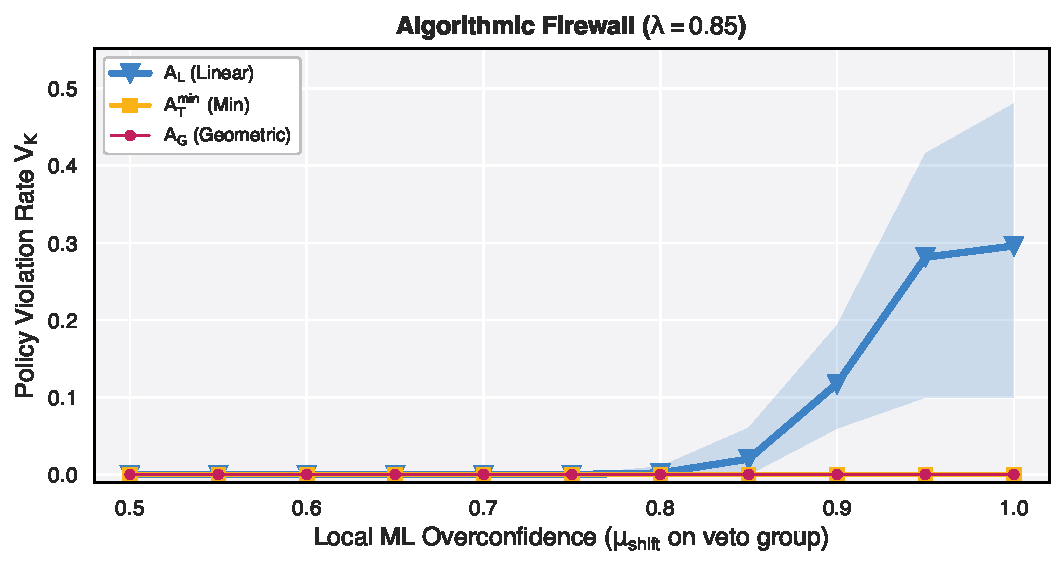
\includegraphics[width=\textwidth]{figures/algorithmic_firewall.pdf}
\caption{Algorithmic firewall under targeted ML overconfidence ($\lambda = 0.85$; $N = 30$ trials). Solid curves: mean; shaded bands: 95\% CI. Operators shown in order $A_L$, $A_T^{\min}$, $A_G$. For $A_L$, $\bar{V}_K$ stays near zero while $\mu_{\text{shift}} \lesssim 0.75$, then rises monotonically to $\bar{V}_K \approx 0.30$ at $\mu_{\text{shift}} = 1.0$ (95\% CI: $[0.10, 0.48]$). $A_T^{\min}$ and $A_G$ maintain $\bar{V}_K = 0$ throughout; the bands collapse to the horizontal axis.}
\label{fig:algorithmic_firewall}
\end{figure}

Figure~\ref{fig:algorithmic_firewall} shows the fragility of compensatory linearity under data-driven prioritization. As the ML layer becomes increasingly overconfident regarding the restricted cases ($\mu_{\text{shift}} \to 1$), $A_L$ allows inflated risk scores to override zero contextual compliance, with $\bar{V}_K \approx 0.30$ on average. Nearly one third of the Top-$K$ tier then consists of institutionally vetoed alternatives. The wide shaded band for $A_L$ reflects substantial trial-to-trial variability in how many vetoed cases breach the cutoff once $\mu_{\text{shift}}$ exceeds $\approx 0.80$. In contrast, both non-linear regimes ($A_T^{\min}$ and $A_G$) maintain $\bar{V}_K = 0$ throughout the adversarial shift in every trial.

This pattern aligns with Proposition~\ref{prop:rank_reversal}: part~(1) explains why $A_L$ admits vetoed alternatives once predictive scores dominate ($\lambda = 0.85$), whereas part~(2) guarantees that conjunctive operators assign $P_i = 0$ whenever $Q_i = 0$, and $A_G$ enforces the same contextual boundary because $Q_i = 0$ zeroes the aggregated score. For CADEMAS designers, these non-linear operators function as an algorithmic firewall that insulates contextual policy from localized predictive failures.

\subsection{Rank Stability Under Contextual Noise}\label{subsect:noise}

Unlike crisp probabilistic outputs, contextual scores $Q_i$ derived from fuzzy rules or human expert evaluations are inherently vague and subject to measurement noise. We measure rank stability as $\bar{\tau}(\sigma)$, the Monte Carlo mean of Kendall's $\tau$ between the ranking at $\sigma = 0$ and the ranking induced under each noise level.

Figure~\ref{fig:noise_propagation} reports $\bar{\tau}(\sigma)$ for $A_L$ and $A_T^{\min}$ at $\lambda = 0.35$; at $\sigma = 0$, both operators reproduce the baseline ranking exactly ($\tau = 1.00$ in every trial).

\begin{figure}[t] 
\centering

\includegraphics[width=\textwidth]{figures/noise_propagation.pdf}
\caption{Rank stability under contextual noise ($\lambda = 0.35$; $N = 30$ trials). Solid curves: mean $\bar{\tau}(\sigma)$; shaded bands: 95\% CI. At $\sigma = 0.5$, $\bar{\tau} \approx 0.40$ for $A_L$ (95\% CI: $[0.38, 0.43]$) vs.\ $\bar{\tau} \approx 0.47$ for $A_T^{\min}$ (95\% CI: $[0.44, 0.50]$); the bands do not overlap, supporting a ranking-stability advantage for the conjunctive operator under moderate vagueness.}
\label{fig:noise_propagation}
\end{figure}

The noise dynamics in Figure~\ref{fig:noise_propagation} extend the homogeneous baseline of Proposition~\ref{prop:cont_homog_rank_preserv}. Once contextual homogeneity is broken by noise, $A_L$ transmits perturbations globally: any fluctuation in $Q_i$ directly perturbs $P_i = \lambda R_i + (1-\lambda) Q_i$, producing a steep decline in $\bar{\tau}$ (from $1.00$ to $\approx 0.40$ at $\sigma = 0.5$). By contrast, $A_T^{\min}$ exhibits selective insensitivity. Whenever $R_i \leq Q_i$, we have $A_T^{\min}(R_i, Q_i) = R_i$, so fluctuations in $Q_i$ above the risk threshold leave $P_i$ unchanged, yielding $\bar{\tau} \approx 0.47$ at $\sigma = 0.5$. In CADEMAS terms, the minimum operator is more robust to vagueness in the contextual modulator when predictive risk already limits the final score.

Taken together, the three experiments in Table~\ref{tab:sim_protocol} show a consistent pattern: non-linear operators enforce contextual boundaries or absorb noise more selectively than $A_L$, whereas linear integration remains efficient only within a bounded $\lambda$ region before governance failures emerge.

\section{Analysis in a More Realistic Case Study}\label{sect:real_example}

The simulations above deliberately use controlled populations so that each failure mode can be observed in isolation. We now ask whether the same operator semantics remain visible in a concrete CADEMAS-ML workflow at resource-constrained scale: the full $n = 100$ employee cohort from the IBM HR Analytics attrition instantiation described by \citet{Godz2026}, with a Top-$K$ tier of $K = 10$ (10\% of the population). Precomputed cooperative risk $R_i$ and context score $Q_i$ are taken from \texttt{experiments/data/attrition100/}\footnote{Files \texttt{cases\_attrition\_100.csv} and \texttt{cases\_attrition\_100\_final.csv}.}.

The cohort contains 100 employees with balanced attrition labels (50 confirmed leavers, 50 stayers) from Research \& Development (56), Sales (40), and Human Resources (4). In CADEMAS-ML terms, $R_i$ aggregates model probabilities or confidences for the positive attrition class across the cooperative ADM units; $Q_i$ is the contextual satisfaction degree under the Digital / Technological Transformation scenario. On this cohort, $R_i \in [0.001, 0.989]$ and $Q_i \in [0, 0.73]$, with 35 employees at $Q_i = 0$ (context veto). The attrition label is retained for verification only and does not enter $P_i$.

We compare five integration settings: $A_L$ at $\lambda = 0.1$ (context-favoring), $\lambda = 0.5$ (balanced baseline, as in \citet{Godz2026}), and $\lambda = 0.9$ (risk-dominated, mirroring the high-$\lambda$ regime in Section~\ref{subsect:opportunity_cost}), together with $A_T^{\min}$ and $A_G$ at $\lambda = 0.5$. We do not include $A_S^{\max}$ here for the same governance reasons as in the simulations. Figure~\ref{fig:real_example_plane} locates all 100 employees in the $(Q_i, R_i)$ plane; Figure~\ref{fig:real_example_bump} traces rank trajectories across the five integration settings for the baseline Top-$K$ tier under $A_L$ ($\lambda = 0.5$, $K = 10$), together with \emph{ghost} entrants---employees outside that baseline list who enter the Top-$K$ tier under at least one non-baseline setting (gray star markers in both figures).

\begin{figure}[t]
\centering   

\includegraphics[width=0.7\textwidth]{figures/real_example_plane.pdf}
\caption{Real attrition example: cooperative risk $R_i$ (ADM probability/confidence for attrition) vs.\ context score $Q_i$ ($n = 100$, Digital Transformation scenario). Grey points are the full cohort; colored circles identify the baseline Top-$K$ tier under $A_L$ ($\lambda = 0.5$, $K = 10$); gray stars mark ghost entrants who reach the Top-$K$ tier under a non-baseline integration setting.}
\label{fig:real_example_plane}
\end{figure}

\begin{figure}[t]
\centering

\includegraphics[width=\textwidth]{figures/real_example_bump.pdf}
\caption{Rank trajectories across $A_L$ at $\lambda = 0.1$, $0.5$, and $0.9$, plus $A_T^{\min}$ and $A_G$ (both at $\lambda = 0.5$), for the baseline Top-$K$ tier under $A_L$ ($\lambda = 0.5$; $n = 100$, $K = 10$). Gray star markers on non-baseline columns indicate ghost entrants; when a ghost ties a baseline employee on $A_T^{\min}$ (e.g., \textit{Lucy Scott} with \textit{Madison Foster} at rank~7, \textit{Richard Johnson} with \textit{Eleanor Foster} at rank~10), the star overlays the baseline circle. Left-column labels report baseline rank and name for ghosts. Employee names appear at the first column only.}
\label{fig:real_example_bump}
\end{figure}

Table~\ref{tab:real_example} lists the baseline Top-$K$ tier and the ten ghost entrants, reporting $R_i$, $Q_i$, aggregated scores, and ranks under all five settings. At the balanced baseline, $A_L$ ($\lambda = 0.5$), $A_T^{\min}$, and $A_G$ agree on the Top-$K$ head: \textit{Laura Baker}, \textit{Andrew Wood}, \textit{Alice Brown}, \textit{Andrew Ross}, and \textit{Caroline Bennett}, each combining elevated cooperative risk with moderate-to-strong context scores. The three operators also agree on the full baseline Top-$K$ list at $\lambda = 0.5$, reflecting a regime where jointly high $R_i$ and $Q_i$ dominate and operator choice is secondary within that tier.

The low-$\lambda$ linear setting inverts that logic. Under $A_L$ with $\lambda = 0.1$, \textit{Julia Smith}---who attains the maximum context score in the cohort ($Q_i = 0.73$) but near-zero cooperative risk ($R_i = 0.005$)---ranks first, ahead of \textit{Laura Baker} and \textit{Andrew Wood}. Under baseline $A_L$ ($\lambda = 0.5$), the same employee falls to rank~48; under $A_T^{\min}$ and $A_G$, $P_i$ collapses toward zero (ranks~55 and~51). Four additional ghosts---\textit{Caroline Adams}, \textit{Caroline Roberts}, \textit{Hunter Adams}, and \textit{Claire Bailey}---similarly enter the Top-$K$ tier only under context-favoring $A_L$, illustrating how fully compensatory linear integration elevates low-probability, high-context profiles that non-linear operators keep far from intervention priority.

The high-$\lambda$ linear setting exposes the compliance failure observed in simulation and highlights the fragility of $A_L$ to the trade-off parameter $\lambda$, especially for vetoed cases. Under $A_L$, any employee with $Q_i = 0$ receives $P_i = \lambda R_i$: cooperative risk enters the priority score in proportion to $\lambda$ even when context excludes the case entirely. In a cohort with 35 context-vetoed employees, this mechanism is dormant at $\lambda = 0.5$---no $Q_i = 0$ case enters the Top-$K$ tier---but becomes operative as $\lambda$ increases. Under $A_L$ with $\lambda = 0.9$, \textit{Camila Phillips}---the highest-$R_i$ employee ($R_i = 0.99$) but context-vetoed ($Q_i = 0$)---rises from rank~26 (baseline $A_L$) to rank~10 and enters the Top-$K$ tier ($P_i = 0.89$). Other vetoed high-risk employees climb in parallel: \textit{Lucas Wright} moves from rank~27 to~13 and \textit{Theodore Adams} from rank~28 to~21, even though they remain outside the intervention tier. Under $A_T^{\min}$ and $A_G$, every vetoed case stays at $P_i = 0$ regardless of $\lambda$. The violation is therefore specific to risk-dominated linear integration, not to the underlying scores. \textit{Amelia Davis} (rank~1 at $\lambda = 0.9$) and \textit{Dominic Collins} (rank~5) further illustrate how increasing $\lambda$ reshuffles the upper tier toward high-$R_i$ profiles even when context scores are weak.

At the opposite extreme, low $\lambda$ makes $A_L$ context-dominated, as noted above for \textit{Julia Smith} and the four context-favoring ghosts. Sweeping $\lambda$ on fixed $(R_i, Q_i)$ pairs thus produces wide rank displacement under $A_L$---from context-prioritized to risk-prioritized orderings---whereas $A_T^{\min}$ and $A_G$ enforce a zero-context boundary and reorder cases through conjunctive or geometric gating rather than through a single compensatory slider.

Ghost behavior under non-linear operators is also informative and exposes tie structures absent under $A_L$. Under $A_T^{\min}$, \textit{Lucy Scott} (ghost; baseline rank~14) enters the Top-$K$ tier at rank~7, tied with baseline employee \textit{Madison Foster}: both share $Q_i = 0.367$ and receive $P_i = \min(R_i, Q_i) = Q_i$, so differentiated cooperative risks ($R_i = 0.87$ vs.\ $0.92$) collapse to the same priority score. At rank~10, \textit{Richard Johnson} (baseline rank~11 under $A_L$) ties \textit{Eleanor Foster} under the same logic ($Q_i = 0.33$, $P_i = 0.33$). In Figure~\ref{fig:real_example_bump}, gray stars overlay the baseline circles at these tied slots on the $A_T^{\min}$ column. Under $A_L$, by contrast, distinct $R_i$ values always yield distinct $P_i$ for a fixed $\lambda$, so such rank-sharing does not arise. \textit{Madison Foster} additionally illustrates linear sensitivity: she remains in the baseline Top-$K$ tier at $\lambda = 0.5$ (rank~10) but drops to rank~37 when $\lambda = 0.9$, displaced by risk-dominated reordering.

These patterns complement the simulation results. Sweeping $\lambda$ on the same observed scores shows how $A_L$ shifts from context-dominated to risk-dominated prioritization---with vetoed cases progressively re-entering contention as $\lambda$ grows---while $A_T^{\min}$ and $A_G$ enforce a zero-context boundary regardless of $\lambda$ and can produce tied rank slots when context is the binding constraint. The bump chart in Figure~\ref{fig:real_example_bump} makes the joint effect of operator choice and $\lambda$ visible for the baseline Top-$K$ tier, its ghost entrants, and the $A_T^{\min}$ ties involving \textit{Lucy Scott} and \textit{Richard Johnson}.

\begin{table}[t]
\centering
\scriptsize
\caption{Baseline Top-$K$ tier and ghost entrants under five integration settings for the 100-case attrition cohort (Digital Transformation scenario, $K = 10$). Superscripts on $P_i$ and $r$ denote the integration setting: $A_L$ at $\lambda = 0.1$, $0.5$, or $0.9$; $A_T^{\min}$ and $A_G$ at $\lambda = 0.5$. Ranks are over all $n = 100$ cases (1 = highest $P_i$). \textbf{Ghost}: enters Top-$K$ under a non-baseline setting while outside the baseline Top-$K$ list.}
\label{tab:real_example}
\setlength{\tabcolsep}{2pt}
\begin{tabular}{lrrrrrrrrrrrrrr}
\toprule
\textbf{Case} & $R_i$ & $Q_i$ & $P_i^{(\lambda=0.1)}$ & $P_i^{(\lambda=0.5)}$ & $P_i^{(\lambda=0.9)}$ & $P_i^{(\min)}$ & $P_i^{(G)}$ & $r^{(\lambda=0.1)}$ & $r^{(\lambda=0.5)}$ & $r^{(\lambda=0.9)}$ & $r^{(\min)}$ & $r^{(G)}$ & \textbf{Ghost} & \textbf{Attr.} \\
\midrule
Laura Baker & 0.9359 & 0.6000 & 0.6336 & 0.7679 & 0.9023 & 0.6000 & 0.7493 & 2 & 1 & 4 & 1 & 1 & No & Yes \\
Andrew Wood & 0.9288 & 0.5667 & 0.6029 & 0.7477 & 0.8925 & 0.5667 & 0.7255 & 3 & 2 & 9 & 2 & 2 & No & Yes \\
Alice Brown & 0.9295 & 0.5600 & 0.5969 & 0.7447 & 0.8925 & 0.5600 & 0.7215 & 4 & 3 & 8 & 3 & 3 & No & Yes \\
Andrew Ross & 0.9302 & 0.4667 & 0.5130 & 0.6984 & 0.8839 & 0.4667 & 0.6589 & 8 & 4 & 17 & 4 & 4 & No & Yes \\
Caroline Bennett & 0.9368 & 0.4571 & 0.5051 & 0.6970 & 0.8888 & 0.4571 & 0.6544 & 9 & 5 & 14 & 5 & 5 & No & Yes \\
Jessica Wilson & 0.9444 & 0.4000 & 0.4544 & 0.6722 & 0.8900 & 0.4000 & 0.6146 & 12 & 6 & 12 & 6 & 6 & No & Yes \\
Noah Murphy & 0.9743 & 0.3600 & 0.4214 & 0.6672 & 0.9129 & 0.3600 & 0.5923 & 15 & 7 & 2 & 9 & 7 & No & Yes \\
Eleanor Foster & 0.9574 & 0.3333 & 0.3957 & 0.6454 & 0.8950 & 0.3333 & 0.5649 & 21 & 8 & 6 & 10 & 10 & No & Yes \\
Christian Bennett & 0.9690 & 0.3200 & 0.3849 & 0.6445 & 0.9041 & 0.3200 & 0.5569 & 24 & 9 & 3 & 12 & 12 & No & Yes \\
Madison Foster & 0.9193 & 0.3667 & 0.4219 & 0.6430 & 0.8641 & 0.3667 & 0.5806 & 14 & 10 & 37 & 7 & 8 & No & Yes \\
\midrule
Leah Cooper & 0.9611 & 0.3000 & 0.3661 & 0.6306 & 0.8950 & 0.3000 & 0.5370 & 26 & 12 & 7 & 13 & 13 & Yes & Yes \\
Amelia Davis & 0.9879 & 0.2667 & 0.3388 & 0.6273 & 0.9158 & 0.2667 & 0.5133 & 28 & 13 & 1 & 14 & 14 & Yes & Yes \\
Lucy Scott & 0.8747 & 0.3667 & 0.4175 & 0.6207 & 0.8239 & 0.3667 & 0.5663 & 18 & 14 & 46 & 7 & 9 & Yes & Yes \\
Dominic Collins & 0.9774 & 0.2000 & 0.2777 & 0.5887 & 0.8996 & 0.2000 & 0.4421 & 38 & 17 & 5 & 17 & 17 & Yes & Yes \\
Camila Phillips & 0.9893 & 0.0000 & 0.0989 & 0.4947 & 0.8904 & 0.0000 & 0.0000 & 62 & 26 & 10 & 66 & 66 & Yes & Yes \\
Julia Smith & 0.0048 & 0.7333 & 0.6605 & 0.3691 & 0.0776 & 0.0048 & 0.0592 & 1 & 48 & 63 & 55 & 51 & Yes & No \\
Caroline Adams & 0.0566 & 0.6000 & 0.5457 & 0.3283 & 0.1109 & 0.0566 & 0.1842 & 5 & 49 & 54 & 32 & 27 & Yes & Yes \\
Caroline Roberts & 0.0203 & 0.6000 & 0.5420 & 0.3102 & 0.0783 & 0.0203 & 0.1104 & 6 & 50 & 62 & 43 & 37 & Yes & No \\
Hunter Adams & 0.0110 & 0.5714 & 0.5154 & 0.2912 & 0.0671 & 0.0110 & 0.0794 & 7 & 51 & 66 & 53 & 42 & Yes & No \\
Claire Bailey & 0.0282 & 0.5333 & 0.4828 & 0.2808 & 0.0787 & 0.0282 & 0.1227 & 10 & 52 & 61 & 39 & 34 & Yes & No \\
\bottomrule
\end{tabular}
\end{table}

\section{Conclusions and Future Directions}\label{sect:conclusions}

This paper examined how the aggregation operator in CADEMAS---a recently proposed cooperative automated decision-making framework \citep{NovoaHernandez2026}---encodes governance semantics when predictive risk and fuzzy contextual knowledge are combined. The theoretical analysis showed that linear integration is fully compensatory: a sufficiently large risk differential can override a weak contextual score (Proposition~\ref{prop:rank_reversal}). The minimum and geometric operators instead enforce hard or softened contextual boundaries, and all monotonic operators preserve the predictive ranking when context is homogeneous across alternatives (Proposition~\ref{prop:cont_homog_rank_preserv}).

The simulation study confirmed that these structural differences have operational consequences. Linear aggregation can remain policy-compliant up to moderate predictive weights while still improving predictive efficiency, but it admits vetoed cases into the Top-$K$ tier once $\lambda$ becomes large. Non-linear operators, especially $A_T^{\min}$ and $A_G$, maintain zero violations under targeted overconfidence and extend the range of data-driven settings available without breaching institutional policy. Under contextual noise, $A_T^{\min}$ preserves rankings more effectively than $A_L$ when cooperative risk already limits the final score. The employee-attrition case study on the full 100-case CADEMAS-ML cohort showed that sweeping $\lambda$ on the same observed scores makes $A_L$ swing from context-dominated to risk-dominated prioritization, with vetoed employees re-entering contention as $\lambda$ increases; ten ghost entrants illustrate how non-baseline settings reorder the intervention tier; $A_T^{\min}$ ties (e.g., \textit{Lucy Scott}--\textit{Madison Foster}, \textit{Richard Johnson}--\textit{Eleanor Foster}) expose rank slots where context alone sets $P_i$; and a context-vetoed employee with maximal $R_i$ enters the Top-$K$ tier only under $A_L$ at $\lambda = 0.9$.

From a governance perspective, the choice of aggregation operator should be treated as a design decision, not a secondary modeling detail. A linear rule signals that predictive and contextual evidence may trade off freely. A minimum rule signals that contextual non-compliance is disqualifying. A geometric rule offers a non-linear compromise with a zero boundary. CADEMAS designers should align this choice with the institutional meaning of $Q_i$ in each application domain.

Several limitations qualify these findings. The Monte Carlo experiments use synthetic populations with stylized veto and noise structures; they isolate failure modes but do not reproduce the joint distribution of real cooperative risk and context scores. The attrition example uses the 100-case IBM HR Analytics CADEMAS-ML pool with precomputed $R_i$ and $Q_i$ rather than retraining the H2O models within this repository. We compared three representative operators rather than the full family of fuzzy t-norms and OWA variants available in the MCDM literature. Finally, the analysis focuses on ranking and Top-$K$ selection; it does not address downstream costs of false negatives, fairness constraints across demographic groups, or dynamic retraining of the predictive layer.

Future work should extend this line of inquiry in four directions. First, replicate the stress tests on additional CADEMAS instantiations and on larger real cohorts with documented policy vetoes. Second, broaden the operator benchmark to include other non-linear families and to study how parameter choice interacts with calibration of $R_i$ and $Q_i$. Third, connect rank stability metrics to decision-theoretic costs (e.g., intervention budget, attrition losses, regulatory penalties) so that operator selection can be evaluated on outcome-relevant grounds. Fourth, integrate aggregation governance into CADEMAS-ML tooling, making operator semantics, compliance thresholds, and sensitivity to noise visible to domain experts during system configuration.

%%%%%%%%%%%%%%%%%%%%%%%%%%%%%%%%%%%%%%%%%%
\authorcontributions{All authors contributed equally to this work. All authors have read and agreed to the published version of the manuscript.}

\funding{This research was supported by the project ``Study, Analysis and Evaluation of Cooperative Automated Decision-Making Systems (CADEMAS)'', PID2023-146575NB-I00, funded by MCIU/AEI/I0.13039/501100011033 and by FSE+. The authors acknowledge support of the previous project.}

\institutionalreview{Not applicable.}

\informedconsent{Not applicable.} 

\dataavailability{Simulation code, figure scripts, and cohort data for the real attrition example are available in the project repository at \url{https://github.com/pnovoahe/cademas-mathematics} (\texttt{experiments/}; 100-case CADEMAS-ML cohort in \texttt{experiments/data/attrition100/}). The underlying IBM HR Analytics dataset is publicly available on Kaggle.} 

\acknowledgments{Mariia Godz has a pre-doctoral research contract associated with the project ``Study, Analysis and Evaluation of Cooperative Automated Decision-Making Systems (CADEMAS)'', PID2023-146575NB-I00, funded by MCIU/AEI/I0.13039/501100011033 and by FSE+. The authors acknowledge support of the previous project.}
 
\conflictsofinterest{The authors declare no conflicts of interest.}

%%%%%%%%%%%%%%%%%%%%%%%%%%%%%%%%%%%%%%%%%%
%% Optional
%\appendixtitles{no} % Leave argument "no" if all appendix headings stay EMPTY (then no dot is printed after "Appendix A"). If the appendix sections contain a heading then change the argument to "yes".
%\appendixstart
%\appendix
%\section[\appendixname~\thesection]{}
%\subsection[\appendixname~\thesubsection]{}

%The appendix is an optional section that can contain details and data supplemental to the main text---for example, explanations of experimental details that would disrupt the flow of the main text but nonetheless remain crucial to understanding and reproducing the research shown; figures of replicates for experiments of which representative data are shown in the main text can be added here if brief, or as Supplementary Materials. Mathematical proofs of results not central to the paper can be added as an appendix.

%\begin{table}[H] 
%\caption{This is a table caption.\label{tab5}}
%\newcolumntype{C}{>{\centering\arraybackslash}X}
%\begin{tabularx}{\textwidth}{CCC}
%\toprule
%\textbf{Title 1}	& \textbf{Title 2}	& \textbf{Title 3}\\
%\midrule
%Entry 1		& Data			& Data\\
%Entry 2		& Data			& Data\\
%\bottomrule
%\end{tabularx}
%\end{table}

%\section[\appendixname~\thesection]{}

%All appendix sections must be cited in the main text. In the appendices, figures, tables, etc., should be labeled starting with “A”, e.g., Figure A1, Figure A2, etc.

%%%%%%%%%%%%%%%%%%%%%%%%%%%%%%%%%%%%%%%%%%
%\isPreprints{}{% This command is only used for ``preprints''.
\begin{adjustwidth}{-\extralength}{0cm}
%} % If the paper is ``preprints'', please uncomment this parenthesis.
%\printendnotes[custom] % Un-comment to print a list of endnotes

\reftitle{References}
\bibliography{biblio.bib}

% If authors have biography, please use the format below
%\section*{Short Biography of Authors}
%\bio
%{\raisebox{-0.35cm}{\includegraphics[width=3.5cm,height=5.3cm,clip,keepaspectratio]{Definitions/author1.pdf}}}
%{\textbf{Firstname Lastname} Biography of first author}
%
%\bio
%{\raisebox{-0.35cm}{\includegraphics[width=3.5cm,height=5.3cm,clip,keepaspectratio]{Definitions/author2.jpg}}}
%{\textbf{Firstname Lastname} Biography of second author}

% For the MDPI journals use author-date citation, please follow the formatting guidelines on http://www.mdpi.com/authors/references
% To cite two works by the same author: \citeauthor{ref-journal-1a} (\citeyear{ref-journal-1a}, \citeyear{ref-journal-1b}). This produces: Whittaker (1967, 1975)
% To cite two works by the same author with specific pages: \citeauthor{ref-journal-3a} (\citeyear{ref-journal-3a}, p. 328; \citeyear{ref-journal-3b}, p.475). This produces: Wong (1999, p. 328; 2000, p. 475)

%%%%%%%%%%%%%%%%%%%%%%%%%%%%%%%%%%%%%%%%%%
%% for journal Sci
%\reviewreports{\\
%Reviewer 1 comments and authors’ response\\
%Reviewer 2 comments and authors’ response\\
%Reviewer 3 comments and authors’ response
%}
%%%%%%%%%%%%%%%%%%%%%%%%%%%%%%%%%%%%%%%%%%
\PublishersNote{}
%\isPreprints{}{% This command is only used for ``preprints''.
\end{adjustwidth}
%} % If the paper is ``preprints'', please uncomment this parenthesis.
\end{document}